\documentclass{main.tex}[subfiles]
\begin{document}
\section{Вычислительные эксперименты}
\subsection{Предобработка данных и выравнивание}
% TODO images

\begin{figure}[H]
    \centering
    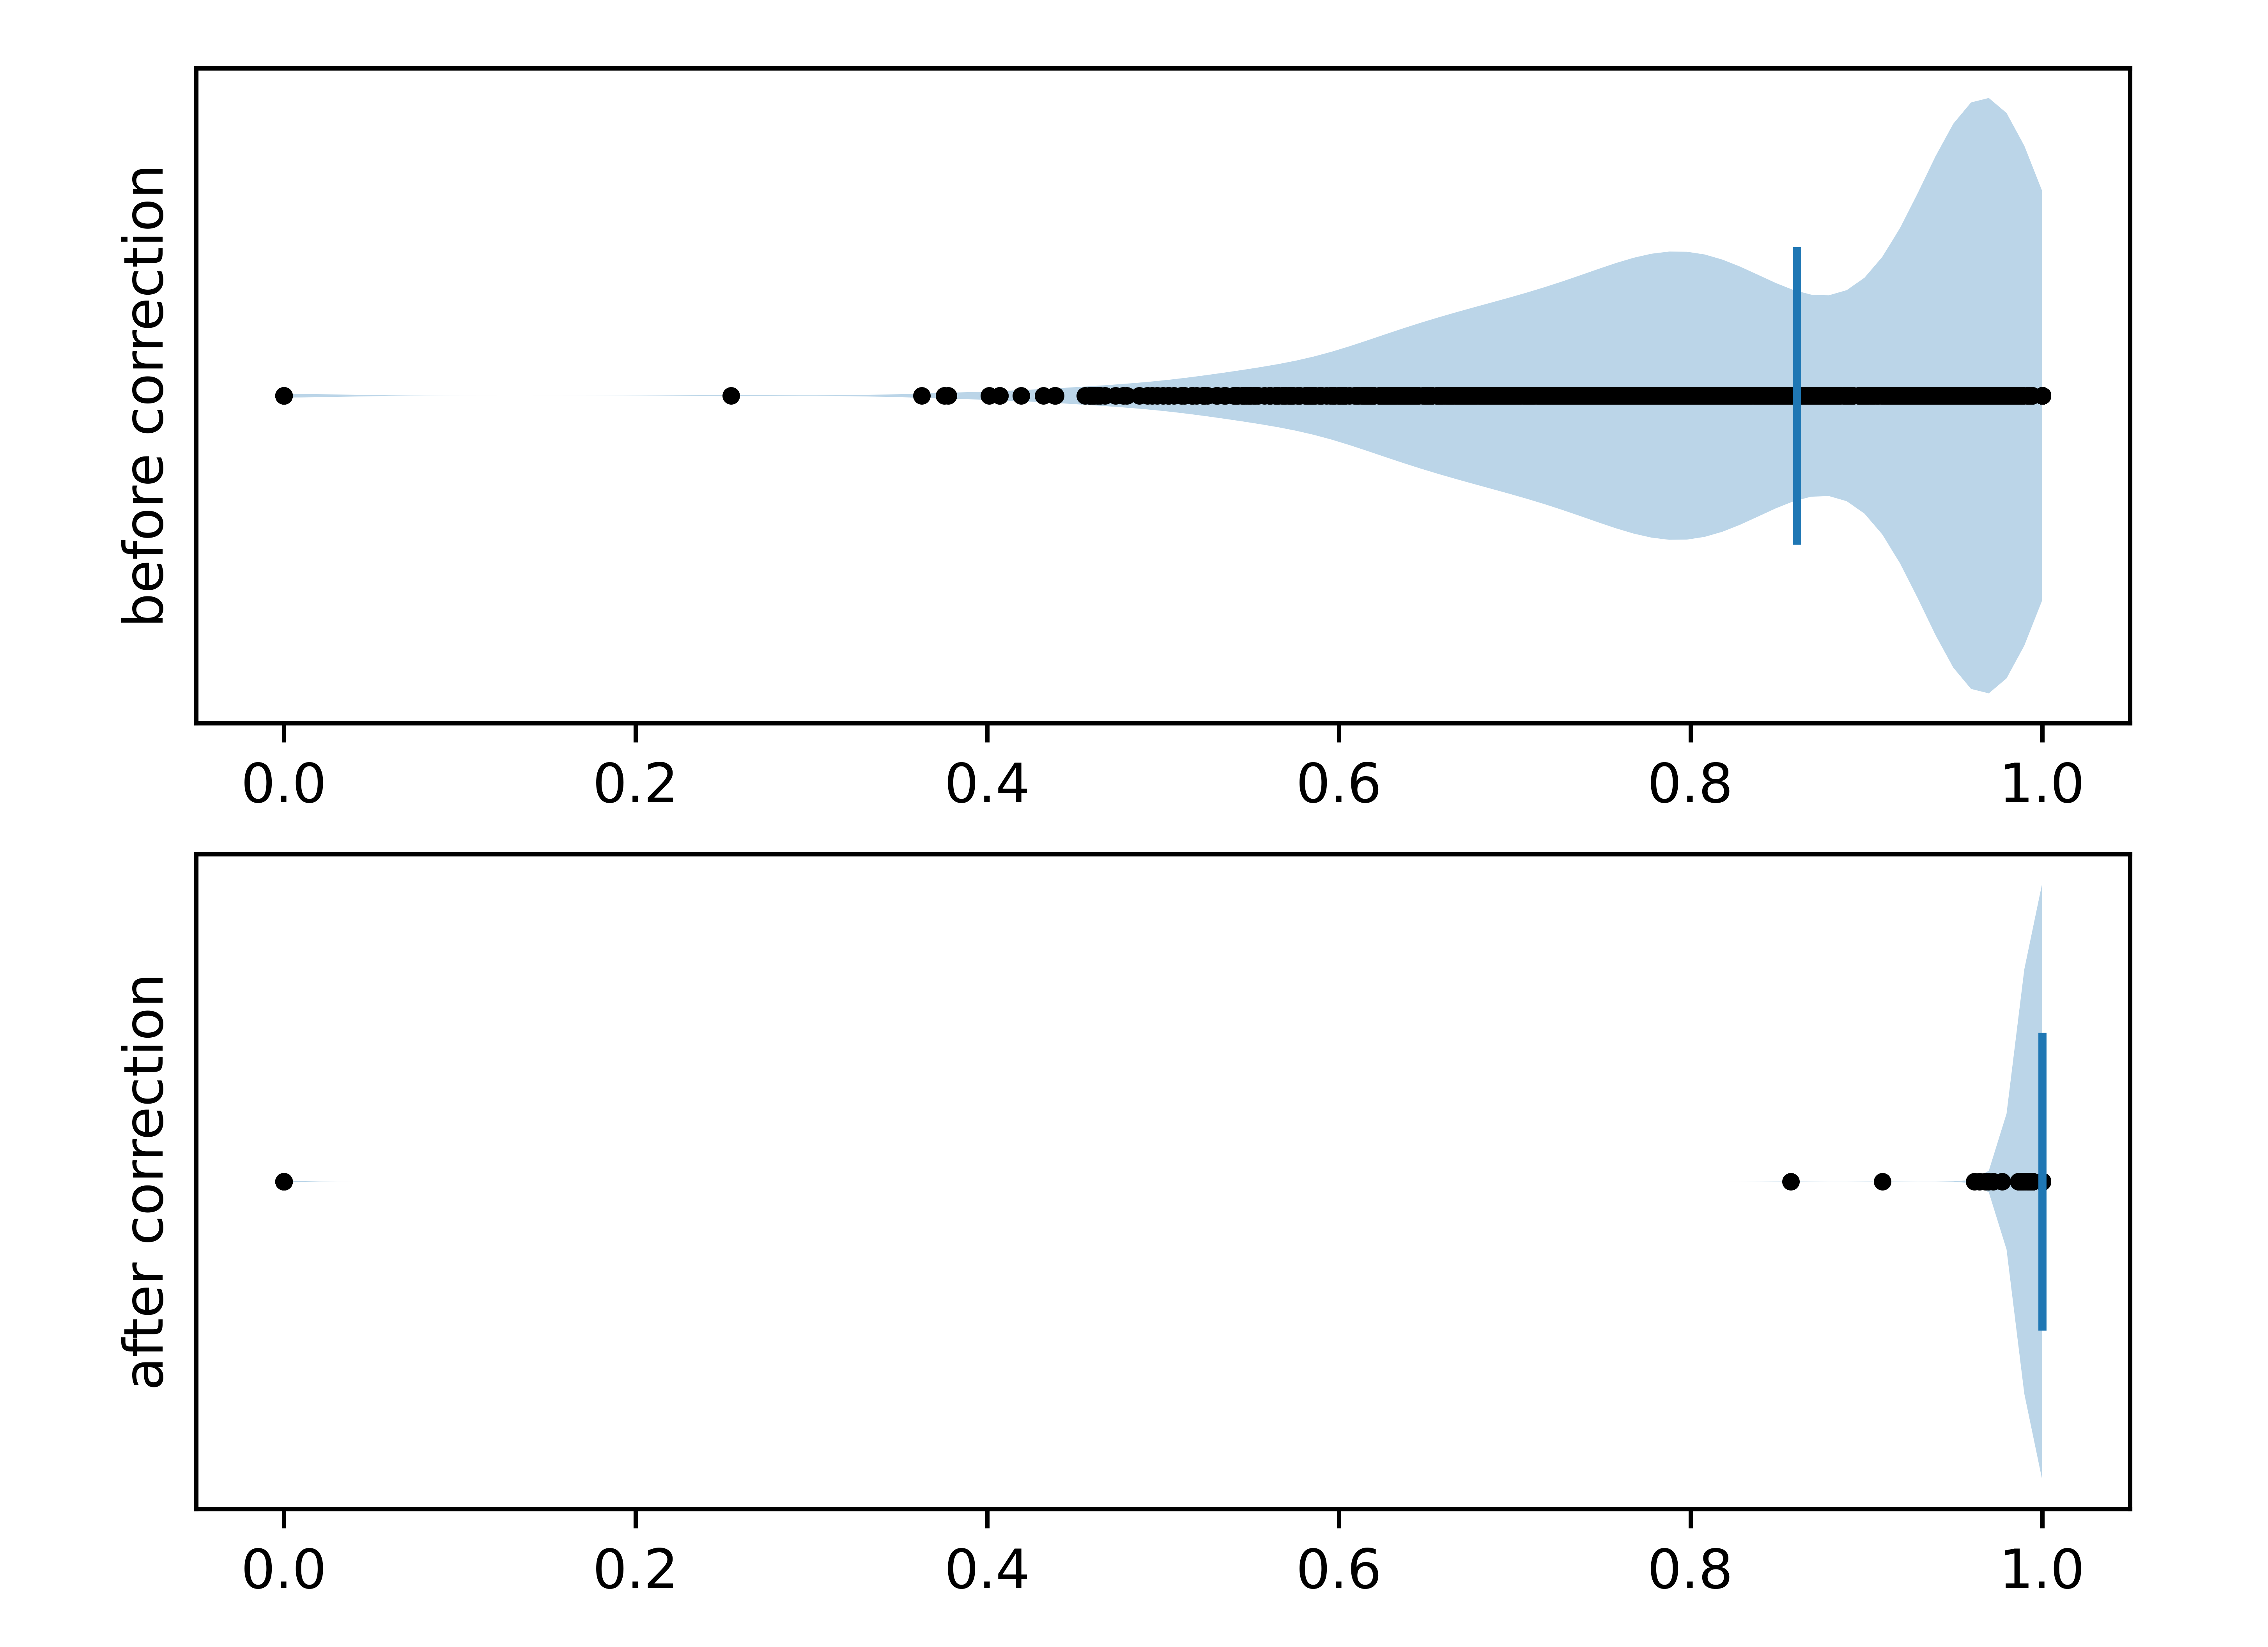
\includegraphics[width=\myPictWidth]{frequencies}
    \caption{Доля слов в распознанном тексте, встречающихся в исходном: до выравнивания (вверху) и после (внизу). Чёрные точки -- элементы выборки, голубая область -- ядерная оценка плотности распределения с ядром Гаусса (т. н. violinplot), синяя вертикальная черта -- медиана выборки}
    \label{fig:frequencies} % TODO ref in the text
\end{figure}

\subsection{Обучение нейронной сети}

% latex table generated in R 4.0.5 by xtable 1.8-4 package
% Sat May 29 22:42:56 2021
\begin{table}[ht]
    \centering
    \caption{Показатели качества обученных моделей (среднее по 3 независимым повторам обучения)}
    \begin{tabular}{llrrr}
        \hline
        валидационный набор & SSL & precision & recall & F1 score \\
        \hline
        \multirow{2}{*}{ Книги (AngelinaDataset) }
         & нет & 0.998 & 0.997 & 0.998 \\
         & да  & 0.996 & 0.994 & 0.995 \\
        \multirow{2}{*}{ Рукописи (AngelinaDataset) }
         & нет & 0.997 & 0.997 & 0.997 \\
         & да  & 0.992 & 0.990 & 0.991 \\
        \multirow{2}{*}{ DSBI }
         & нет & 0.997 & 0.995 & 0.996 \\
         & да & 0.986 & 0.989 & 0.987 \\
        \multirow{2}{*}{ Книги с псевдометками }
         & нет & 0.817 & 0.111 & 0.194 \\
         & да & 0.982 & 0.989 & 0.986 \\
        \hline
    \end{tabular}
    \label{table:validate_results} % TODO ref in the text
\end{table}


\end{document}